% Author: Mathias Hablützel

\section{Erfassung Windfelder}\label{s:windfields}

\subsection{Problemanalyse}
\subsubsection{Einlesen der Daten}
Die vorgegebenen Inputdaten in einer einfachen, unstrukturierten Text-Datei
werden als Vektor eingelesen, zwei numerische Werte werden jeweils als $u$-
bzw. $v$-Komponente an einer bestimmten Position erfasst.

\subsubsection{Verwalten der Daten}
Da pro bestimmten Zeitpunkt ein bekanntes (prognostiziertes) Windfeld bekannt
ist, müssen mehrere Windfelder verwaltet werden können. Es kann der Fall
eintreten, an dem der Windvektor $a_{x,y,t}$ und der Windvektor einer
unmittelbar daneben liegenden Position an einem etwas späteren Zeitpunkt
gebraucht wird, also $a_{x+1,y,t+1}$ zum Beispiel. Somit müssen die
Positionsangaben vom Windfeld zu $t$ und $t+1$ identisch sein. 

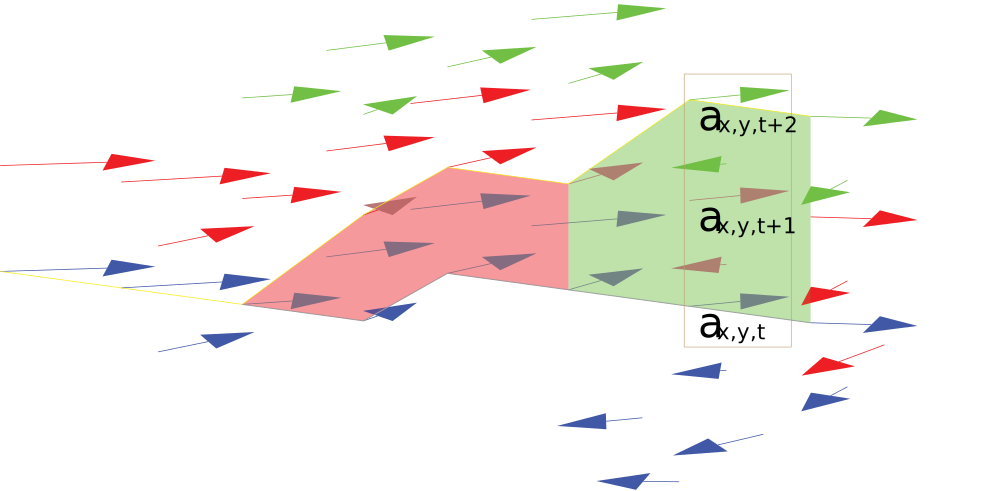
\includegraphics[width=12cm]{img/windfield-different-layer}
